\subsection{4 Laufrichtungen}

\subsubsection{Versuch 7}
Die Charaktersteuerung benötigt je nach Tastatureingabe eine der vier Bewegungsrichtungen. Der Unity ML-Agents Agent enthält eine Funktion zum wechseln des verwendeten Modells. Mit dieser Funktion wird in folgender Implementierung zwischen den Modellen aus Versuch 6 gewechselt um alle Bewegungsrichtungen mit einer Steuerung abzudecken. Zu Erwarten ist das die Bewegung in die einzelnen Richtungen funktioniert, der Läufer aber beim Wechsel zwischen den Modellen das Gleichgewicht nicht halten kann.

\begin{lstlisting}[caption={Laufrichtung Modell wechseln},captionpos=b,label={lst:laufrichtung_modell_wechsel}]
public override void FixedUpdate() {
    ...    
    agent.targetWalkingSpeed = 5f;
    if (inputVert != 0) //Tastatur Input Vor oder Zurück
    {
        // Vorwärts
        if (inputVert > 0)
        {
            agent.SetModel("Walker", modelForward);
        }
        else // Zurück
        {
            agent.SetModel("Walker", modelBackward);
        }
    }
    else if (inputHor != 0) // Links oder Rechts
    {
        if (inputHor > 0) // Rechts
        {
            agent.SetModel("Walker", modelRight);
        }
        else // Links
        {
            agent.SetModel("Walker", modelLeft);
        }
    }
    else //kein Input -> Auf der Stelle stehen
    {
        agent.targetWalkingSpeed = 0f;
        agent.SetModel("Walker", modelStanding);
    }
    ...
}
\end{lstlisting}

Wie angenommen funktioniert das Bewegen in eine konstante Richtung gut. Beim Wechsel zu einem anderen Modell fällt der Läufer ohne Ausnahme.

\subsubsection{Versuch 8}
In Versuch 8 wird die Möglichkeit geprüft, alle Bewegungsrichtungen in einem Modell anzulernen. Dafür wird zum Start eine zufällige Bewegungsrichtung für jeden Läufer ausgewählt, mit dem Ziel das die Läufer direkt mit unterschiedliche Bewegungsrichtungen trainieren. Das gleichzeitige trainieren mit mehreren Läufern und unterschiedlichen Gehrichtungen soll das erlernen einer generell gültigen Strategie fördern. Die Gehrichtung wechselt beim erreichen eines Ziels, damit soll erreicht werden das der Läufer das aktuelle Ziel mit ausgewählter Bewegungsrichtung vollständig erlernt. Durch das öftere erreichen von Zielen im Verlauf des Trainings wird aber auch gleichzeitig jede beliebige Kombination angelernt. Als Ausgleich in der Komplexität wird die Zielgeschwindigkeit für das ganze Training festgesetzt.

\begin{lstlisting}[caption={Laufrichtung zufällig zum Start und beim erreichen von Ziel},captionpos=b,label={lst:laufrichtung_wechsel_start_ziel}]
public Direction direction = Direction.Forward;
Direction[] directions;

public override void Initialize()
{
    ...
    directions = (Direction[])Enum.GetValues(typeof(Direction));
    SetRandomWalkDirection();
    onTouchedTarget.AddListener(SetRandomWalkDirection);
}

public void SetRandomWalkDirection()
{
    direction = directions[Random.Range(0, directions.Length)];
}

public override void CollectObservations(VectorSensor sensor)
    {
        ...
        sensor.AddObservation((float)direction);
    }
\end{lstlisting}

Codeausschnitt \ref{lst:laufrichtung_wechsel_start_ziel} erstellt beim Initialisieren des Agenten ein Array mit allen Werten, welche das Richtungs-Enum zulässt. Die Funktion SetRandomWalkDirection wählt eine zufällige Richtung aus und setzt diese für den Agenten. Die Funktion wird zu Beginn in Initialize aufgerufe. Zusätzlich wird die Methode mit einem Listener auf das onTouchedTarget des Agenten registriert. Die Methode wird somit bei jedem berühren eines Ziels ausgeführt. Das der Agent während dem Training sowie nach dem Training zwischen den Laufrichtungen entscheiden kann, bekommt er einen Zahlenwert repräsentativ für die Richtung in der Beobachtung angehängt.

Der Läufer lernt unter diesen Bedingungen sehr langsam und das Training stagniert. Ab ca. 20 millionen Trainingsschritten fängt der Läufer an regelmäßig Ziele zu erreichen. Durch das häufige erreichen von Zielen steigt aber auch die Anzahl der Ziel- und Laufrichtungswechsel. Aus diesem Grund brechen die Belohnungen ein und der Fortschritt stagniert (siehe Abbildung \ref{fig:versuch8_training}).

\begin{figure}[H]
  \centering  
  \begin{subfigure}{.49\textwidth}
      \centering  
      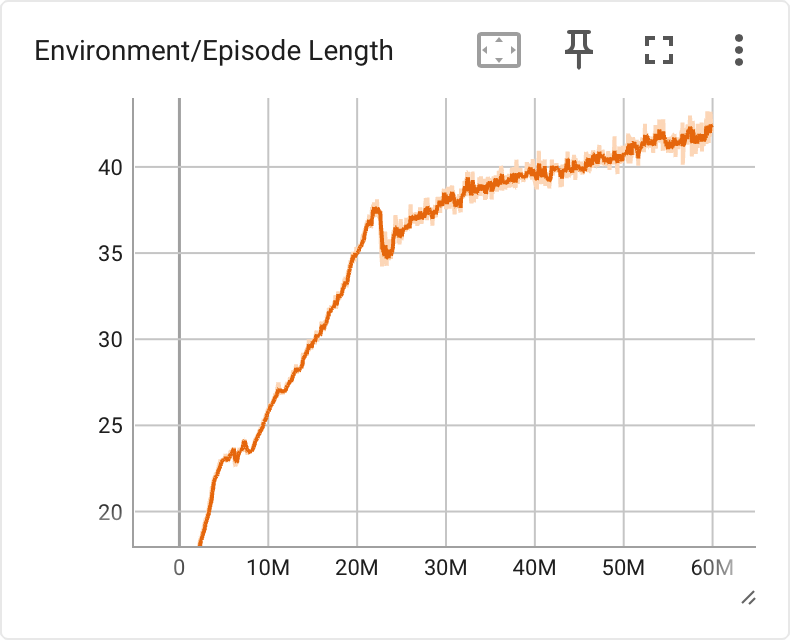
\includegraphics[width=\textwidth]{img/134_episode_length}
      \caption{Episodenlänge}
      \label{fig:134_episode_length}
    \end{subfigure}
    \begin{subfigure}{.49\textwidth}
      \centering  
      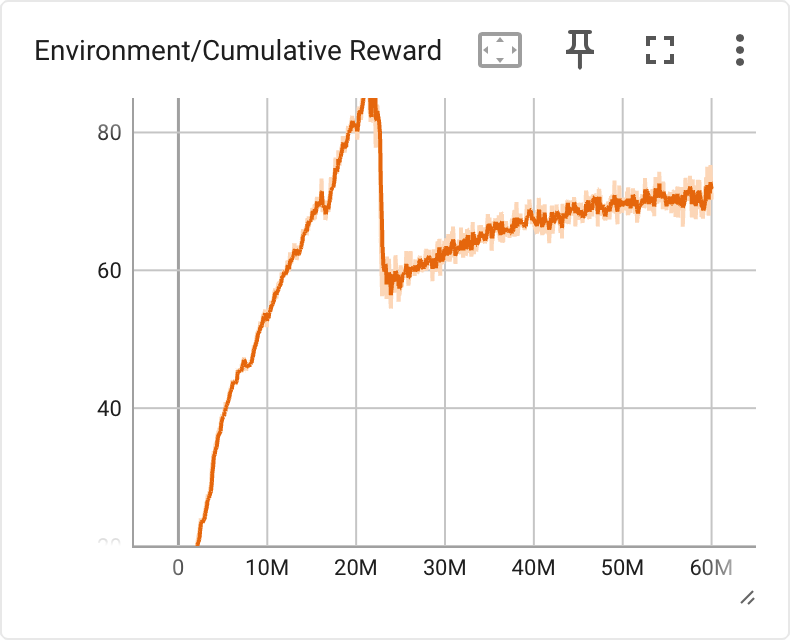
\includegraphics[width=\textwidth]{img/134_cumulative_reward}
      \caption{Angehäufte Belohnung}
      \label{fig:134_cumulative_reward}
    \end{subfigure}
     \begin{subfigure}{.49\textwidth}
      \centering  
      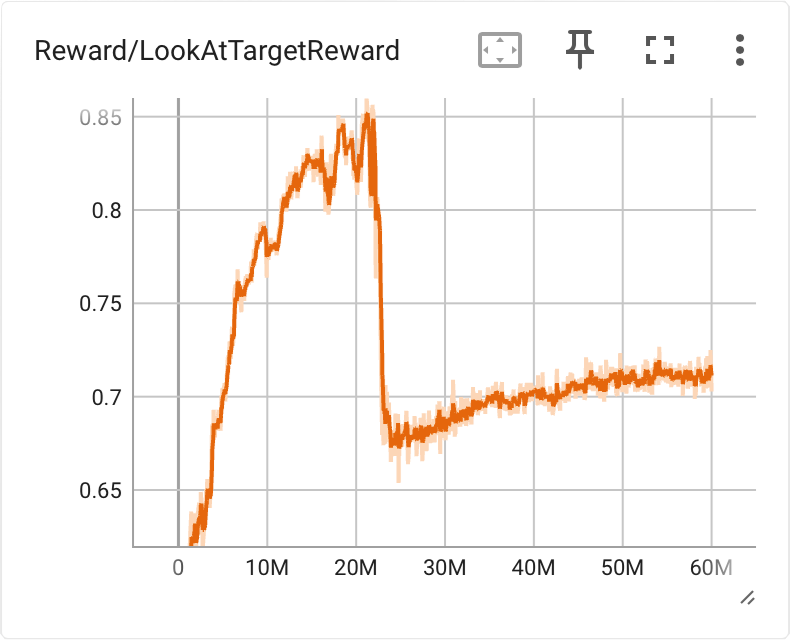
\includegraphics[width=\textwidth]{img/134_look_reward}
      \caption{Blickbelohnung}
      \label{fig:134_look_reward}
    \end{subfigure}
    \begin{subfigure}{.49\textwidth}
      \centering  
      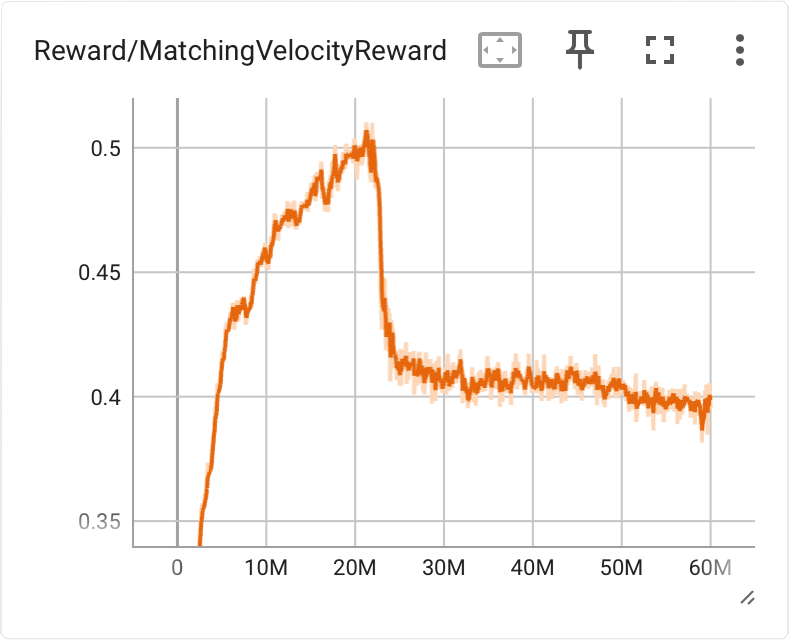
\includegraphics[width=\textwidth]{img/134_vel_reward}
      \caption{Geschwindigkeitsbelohnung}
      \label{fig:134_vel_reward}
    \end{subfigure}
    \begin{subfigure}{.49\textwidth}
      \centering  
      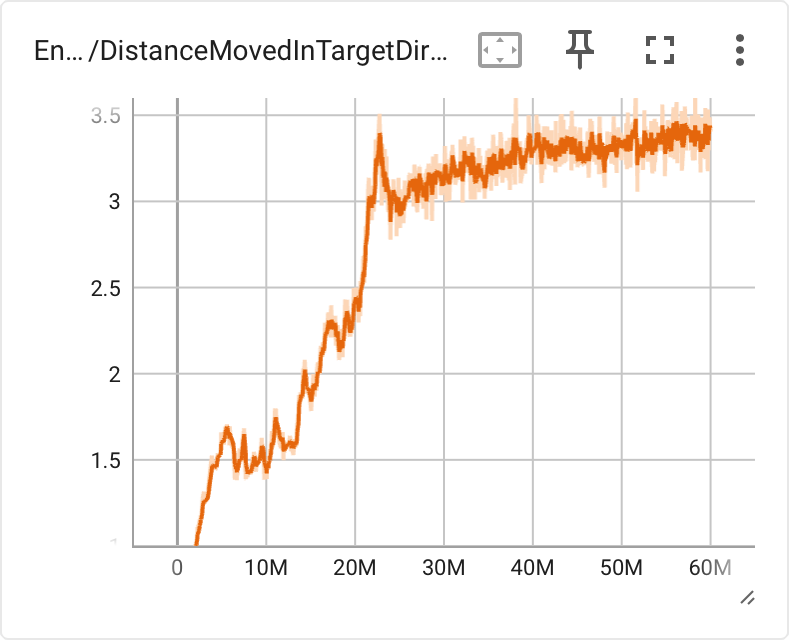
\includegraphics[width=\textwidth]{img/134_move_target_dir}
      \caption{Zurückgelegte Stecke in Zielrichtung}
      \label{fig:134_move_target_dir}
    \end{subfigure}
    \begin{subfigure}{.49\textwidth}
      \centering  
      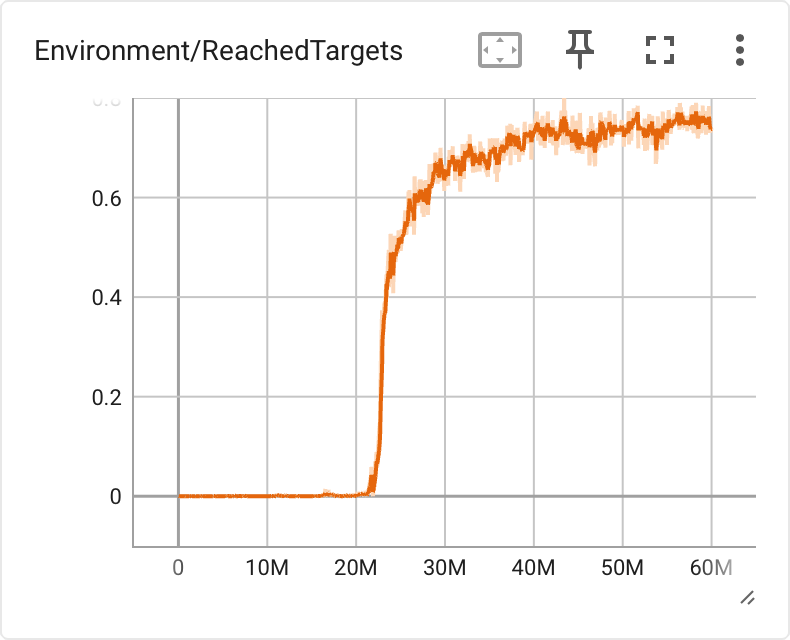
\includegraphics[width=\textwidth]{img/134_reach_target}
      \caption{Anzahl erreichte Ziele}
      \label{fig:134_reach_target}
    \end{subfigure}
  \caption{Versuch 8 Training Graphen}
  \label{fig:versuch8_training}
\end{figure}

\subsubsection{Versuch 9}
Um den Richtungswechsel regelmäßiger zu gestalten, wird getestet wie das Training sich verhält wenn die Richtung beim Start jeder neuen Trainingsepisode zufällig gewählt wird.

\begin{figure}[H]
  \centering  
  \begin{subfigure}{.49\textwidth}
      \centering  
      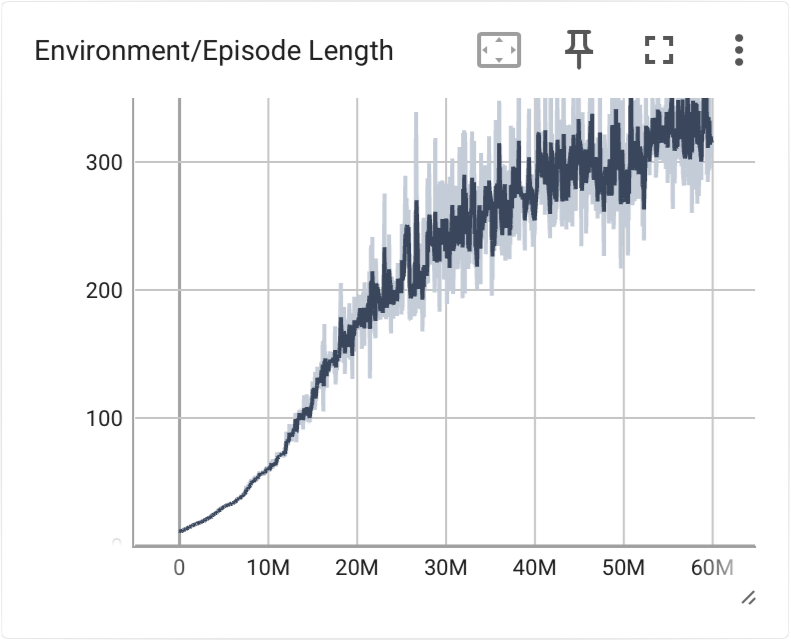
\includegraphics[width=\textwidth]{img/135_episode_length}
      \caption{Episodenlänge}
      \label{fig:135_episode_length}
    \end{subfigure}
    \begin{subfigure}{.49\textwidth}
      \centering  
      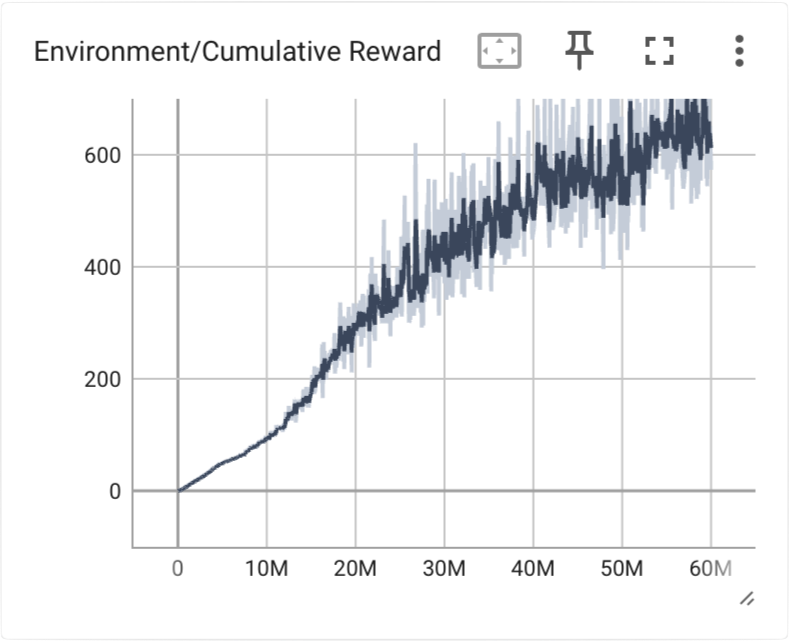
\includegraphics[width=\textwidth]{img/135_cumulative_reward}
      \caption{Angehäufte Belohnung}
      \label{fig:135_cumulative_reward}
    \end{subfigure}
     \begin{subfigure}{.49\textwidth}
      \centering  
      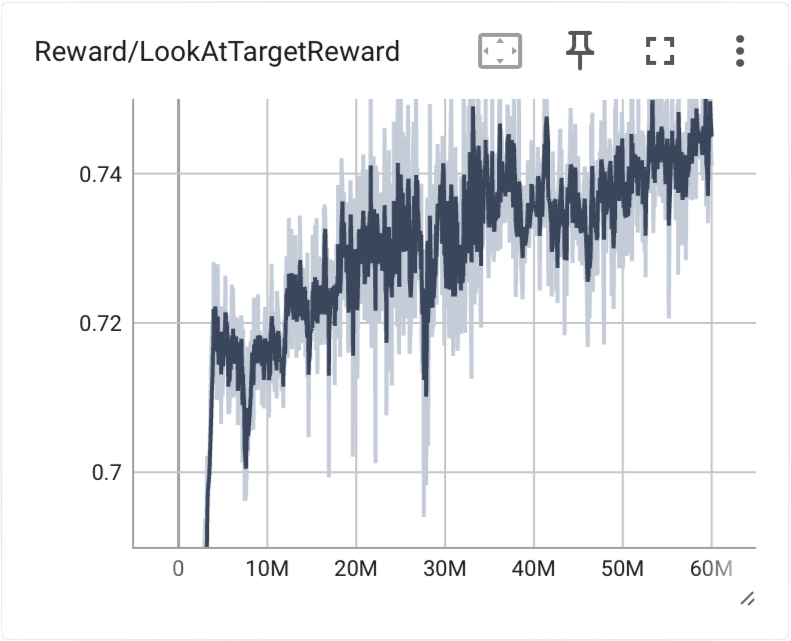
\includegraphics[width=\textwidth]{img/135_look_reward}
      \caption{Blickbelohnung}
      \label{fig:135_look_reward}
    \end{subfigure}
    \begin{subfigure}{.49\textwidth}
      \centering  
      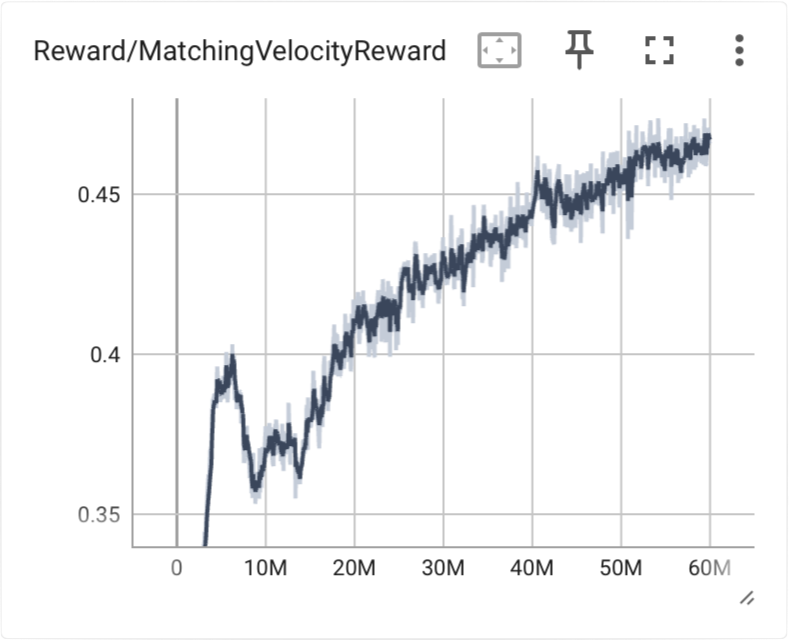
\includegraphics[width=\textwidth]{img/135_vel_reward}
      \caption{Geschwindigkeitsbelohnung}
      \label{fig:135_vel_reward}
    \end{subfigure}
    \begin{subfigure}{.49\textwidth}
      \centering  
      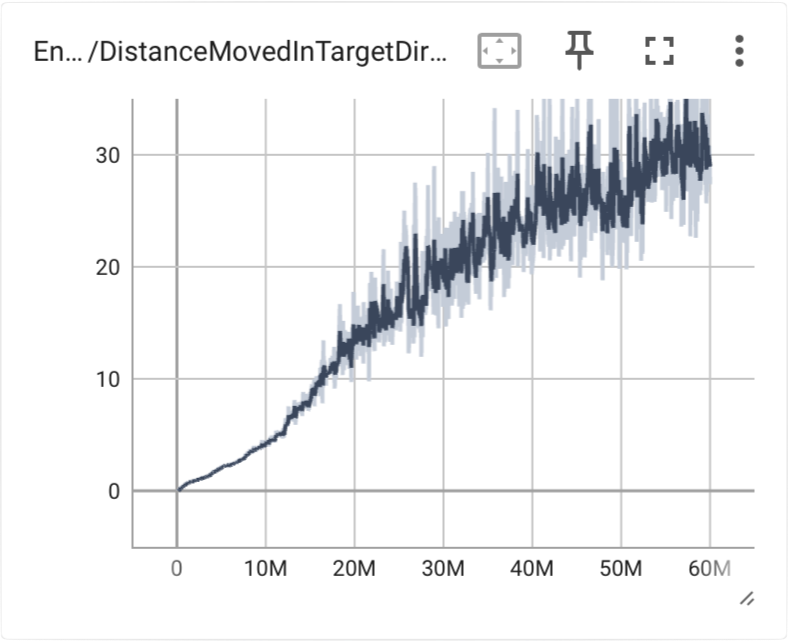
\includegraphics[width=\textwidth]{img/135_move_target_dir}
      \caption{Zurückgelegte Stecke in Zielrichtung}
      \label{fig:135_move_target_dir}
    \end{subfigure}
    \begin{subfigure}{.49\textwidth}
      \centering  
      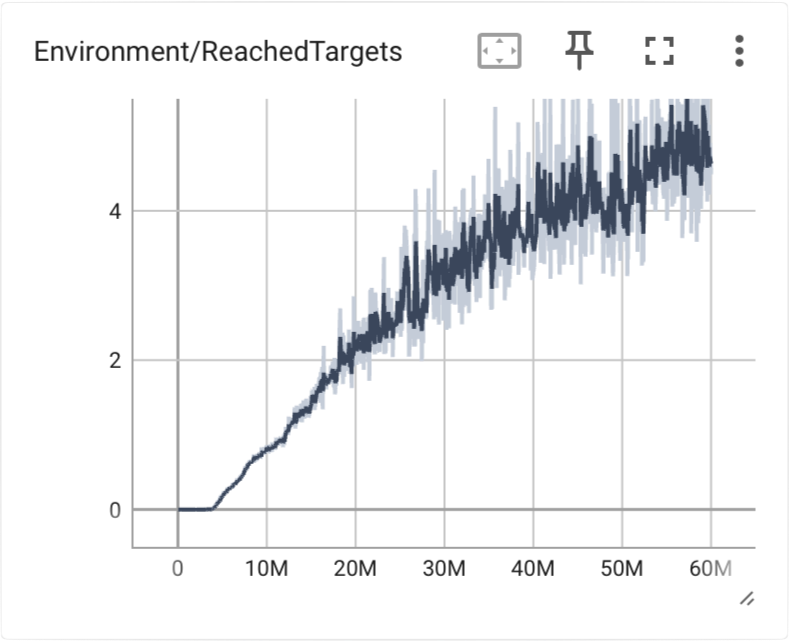
\includegraphics[width=\textwidth]{img/135_reach_target}
      \caption{Anzahl erreichte Ziele}
      \label{fig:135_reach_target}
    \end{subfigure}
  \caption{Versuch 9 Training Graphen}
  \label{fig:versuch9_training}
\end{figure}

Das gleichbleiben der Laufbewegung über die komplette Trainingsepisode hat zur folge dass das Training stabiler verläuft siehe Abbildung \ref{fig:versuch9_training}. Der Nachteil ist jedoch das der Läufer keine Bewegungswechsel lernt. Beim steuern des Läufers ist das wechseln zwischen den Laufrichtungen noch immer ein Problem. Dazu kommt das der in diesem training die Blickrichtungs Belohnung geringer ist als bei vorherigen Trainingseinheiten. Der Läufer lernt die seitwärts Bewegungen nicht richtig sondern nimmt einen Verlust in der Belohnung in kauf für die Steigerung der Episodenlänge.